\chapter{XFlowRL: Reinforcement Learning Optimisation}
In this chapter we will introduce the graph optimisation problem and describe the technical details of the design of the two reinforcement learning agents and their components in relation to prior work. Furthermore, we will frame the optimisation problem in the RL domain by describing the system environment, the reward calculation and the state-action space. Additionally, we describe the RL agents trained in the model-free and model-based domains as well as highlighting limitations in the application of reinforcement learning to this problem. Finally, we discuss the relative benefits of each approach as well as the significant challenges that we must overcome to apply RL to this problem and establish the baselines to compare the model-free and model-based agents.

\section{Graph-level optimisation}

Performing optimisations at a higher, graph-level means that the resulting graph is---in terms of execution methodology---no different than the original graph prior to optimisation. Therefore, by performing graph-level optimisation we generate a platform and backend independent graph representation which can be further optimised by specialised software for custom hardware accelerators such as GPUs and TPUs.

Next, we define that two computation graphs, $\mathcal{G}$ and $\mathcal{G}'$ are semantically equivalent when $\forall \mathcal{I} : \mathcal{G}(\mathcal{I}) = \mathcal{G}'(\mathcal{I})$ where $\mathcal{I}$ is an arbitrary input tensor. We aim to find the optimal graph $\mathcal{G}^*$ that minimises the cost function, \texttt{cost}$(\mathcal{G})$, by performing a series of transformations to the computation graph at each step, the specific transformation applied does not need to be strictly optimal. In fact, by applying optimisations that reduce graph runtime we further increase the state space for the search; a large state space is preferable in the reinforcement learning domain.

An important problem in graph-level optimisation is that of defining a set of varied, applicable transformations that can be used to optimise the graphs. As previously noted, prior work such as TensorFlow use a manually defined set of transformations and optimise greedily. On the other hand, TASO uses a fully automatic method to generate candidate transformations by performing a hash-based enumeration over all possible DNN operators that result in a semantically equivalent computation graph.

\begin{figure}[htbp]
  % preliminary
  \sbox\twosubbox{%
    \resizebox{\dimexpr.9\textwidth-1em}{!}{%
      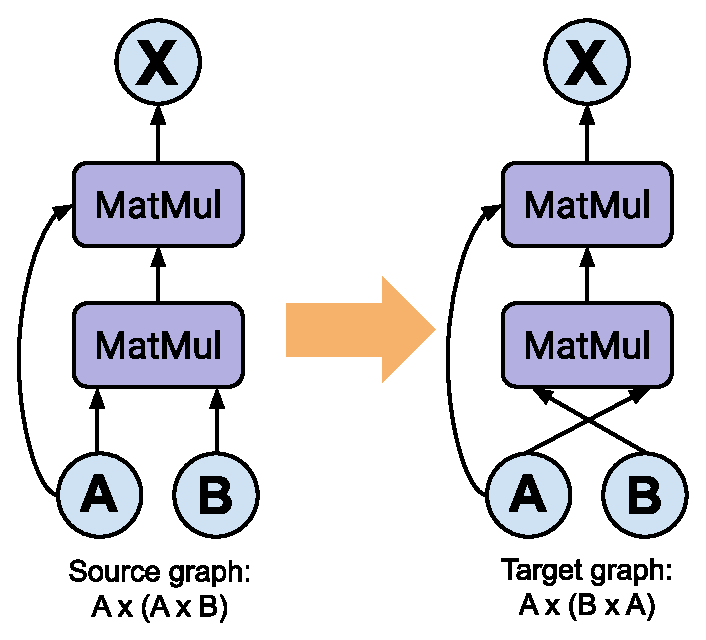
\includegraphics[height=3cm]{sections/3problem/images/rewrite1}%
      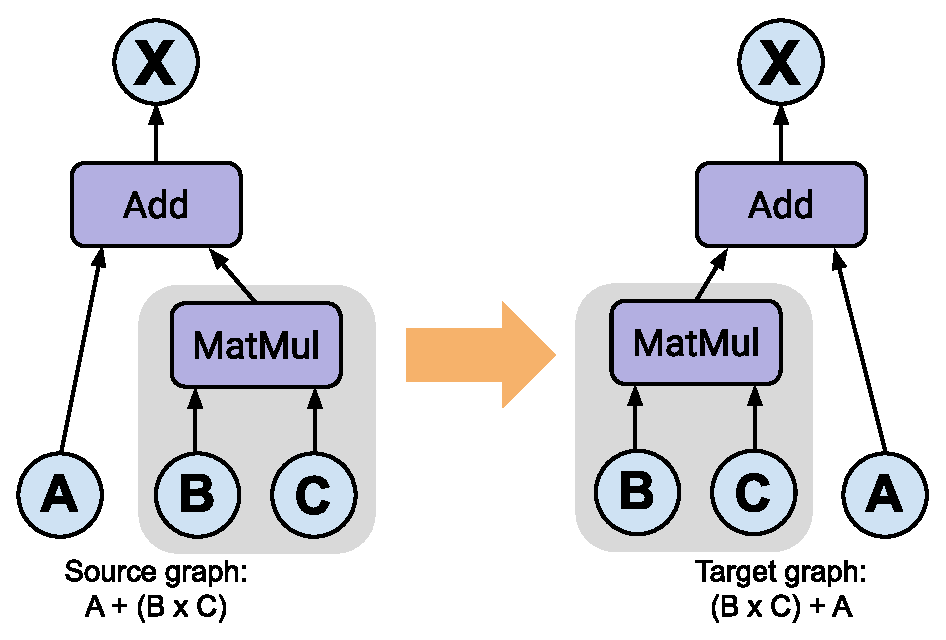
\includegraphics[height=3cm]{sections/3problem/images/rewrite2}%
    }%
  }
  \setlength{\twosubht}{\ht\twosubbox}
  
  % typeset
  \centering
  \subcaptionbox{Tensor renaming substitution \label{fig:problem:rewrite-graph1}}{
    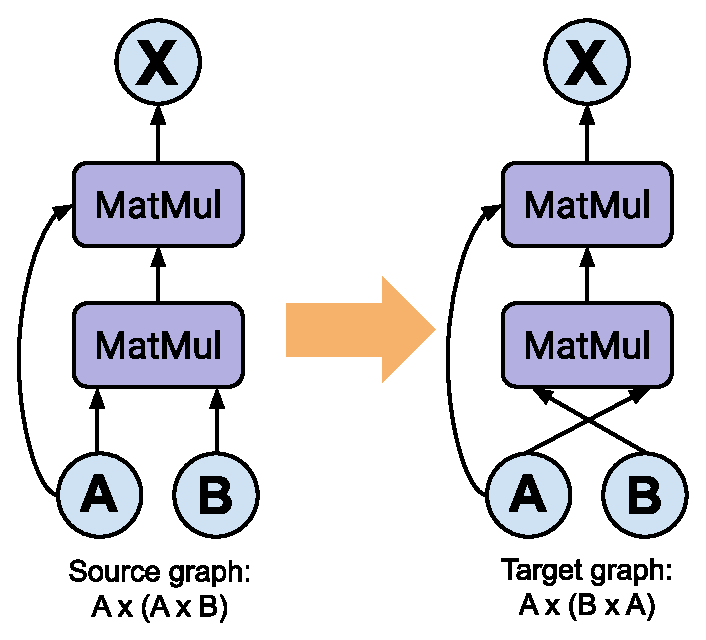
\includegraphics[height=\twosubht]{sections/3problem/images/rewrite1}
  }\quad
  \subcaptionbox{Common subgraph substitution \label{fig:problem:rewrite-graph2}}{
    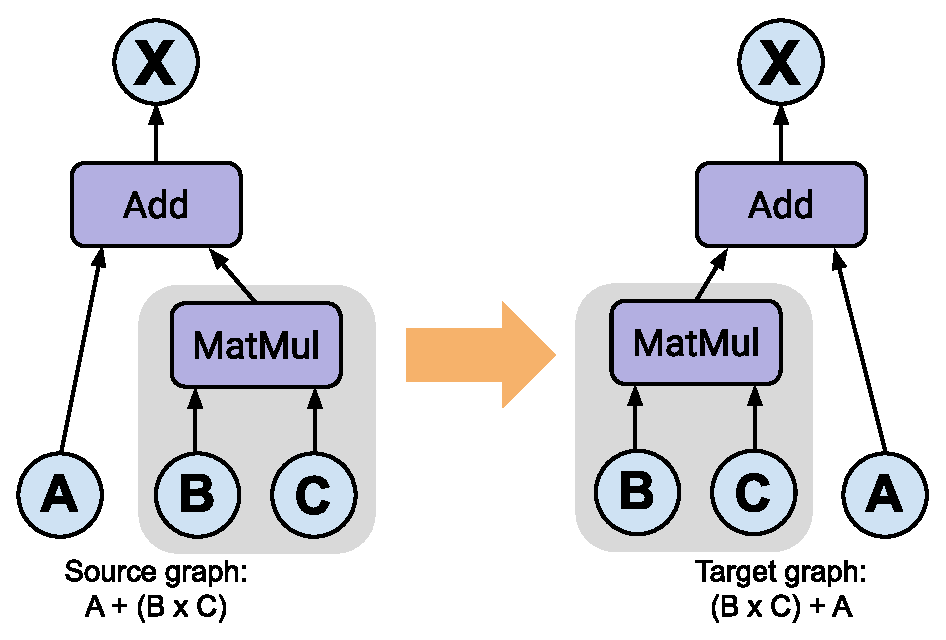
\includegraphics[height=\twosubht]{sections/3problem/images/rewrite2}
  }
  \caption[Two examples of trivial graph substitutions]{Two examples of trivial graph substitutions that does not impact the overall runtime of the computation graph. The left sub-figure shows a simple renaming of the tensor inputs. The figure on the right shows that we have a common sub-graph between the source and the target graphs. In both cases we eliminate the duplicates as the hash of the two graphs will be identical.}
\end{figure}

In this work, we take the same approach as that of TASO and automatically generate the candidate graphs. We perform this as an offline step as it requires a large amount of computation to both generate and verify the candidate substitution; to place an upper bound on the computation, we limit the input tensor size to a maximum of 4x4x4x4 during the verification process. Following the generation and verification steps, we prune the collection to remove substitutions that are considered trivial and as such would not impact runtime. For example, trivial substitutions include input tensor renaming and common subgraphs, we show both techniques diagrammatically in Figure \ref{fig:problem:rewrite-graph1} and \ref{fig:problem:rewrite-graph2} respectively.

\subsection{Graph Embedding}
\label{sec:design:subsec:embed}
% As we described in the previous section, the reinforcement learning agent must learn to choose two actions at each step in an epoch; the transformation and location from the set available dependent on the current computation graph. To learn the optimal action selection, we must create an embedding from the computation graph representation in the machine learning framework to our internal, manipulable graph representation inside our environment, our modified TASO backend.

When developing the project, a pivotal part of the project is the decision as the representation of the GNN as there are a wide variety of forms which it can take. For example, a common implementation are message-passing networks (MPNNs) \cite{gilmer2017neural} which reduce data along edges and between nodes in the graph. Alternatively, we considered using graph convolutional networks (GCNs) \cite{kipf2016semi}, however, we found that using messages passing networks produced a more generalisable embedding as we leverage the relational biases in the graph structure and avoid imposing restrictions on the learned embedding accidentally.

[TODO] cite related work that used GNNs in Computer Systems

During training of the reinforcement learning agents, we convert the internal graph representation to a graph neural network. In order to train the model-free and model-based agents, a latent space embedding of the computation graph is required. Therefore, using the \texttt{graph\textunderscore nets} package developed by Battaglia et al. \cite{battaglia2018relational}, we use the graph neural network to learn a latent space embedding of the graph using message passing networks to gather the global learned features of the graph.

[TODO also describe the embedding parameters for graph network]

Furthermore, we acknowledge the work by Kai Fricke and Michael Schaarschmidt who developed the initial Python interface with TASO, the algorithm for converting the C++ TASO graph representation into a Cython object and performed experiments a model-free reinforcement learning agent \cite{xflowrl2019}. We used their work as a foundation upon which we continued development and research into model-free and model-based RL.


\section{Reinforcement Learning formulation}
In the following section we will describe how to represent the computation graph optimisation problem in the reinforcement learning domain by describing the key components of the system. We describe the system environment in which the agents act, the state-action space, and finally the reward functions for both the model-free and model-based agents which we used to determine the optimal reward signal to train the agents.

\subsection{System environment}
\label{sec:prob:subsec:sysenv}

In order to train a reinforcement learning agent, it necessary that we have access to an environment that, given the current environment state, the agent can take an action. After taking the chosen action, the environment is updated into a new state and the agent receives a reward signal. Typically, one uses a mature environment such as OpenAI Gym \cite{brockman2016openai} or OpenSpiel \cite{LanctotEtAl2019OpenSpiel} as the quality of the environment often has a significant effect on the stability of training. Moreover, using an environment that uses a common interface allows researchers to implement algorithms with ease and, importantly, reproduce results from published conference papers.

In our work, we implemented an environment that follows the OpenAI Gym API standard stepping an environment, that is, we have a function \texttt{step(action)} that accepts a single parameter, the action requested by the agent to be performed in the environment. The \texttt{step} function returns a 4-tuple \texttt{(next\textunderscore state, reward, terminal, extra\textunderscore info)}. \texttt{extra\textunderscore info} is a dictionary which can store arbitrary data. The environment in our project has a structure that is shown diagrammatically in figure \ref{fig:problem:sys-env}.

\begin{figure}[ht]
  \centering
  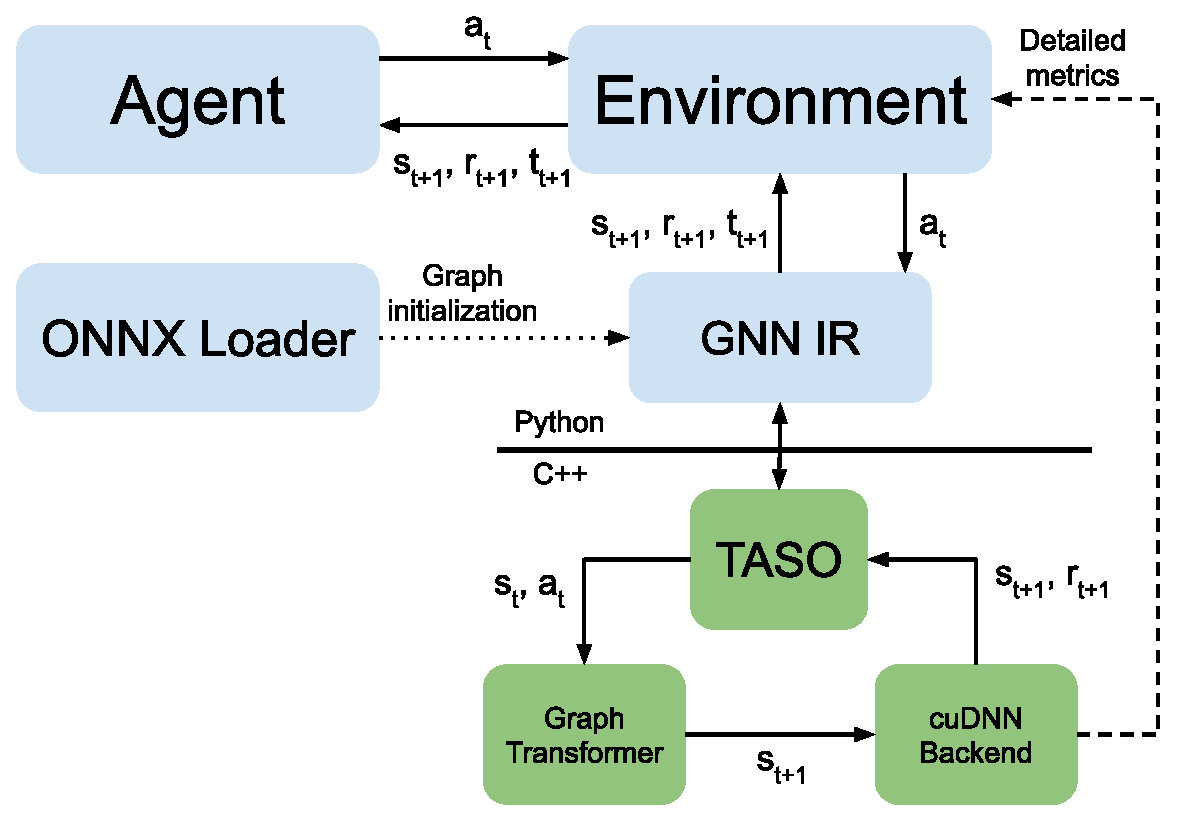
\includegraphics[width=0.75\columnwidth]{sections/3problem/images/sysenv}
  \caption[RL system environment]{Data flow between components of the RL system. Although this diagram shows the setup for both the training of the model-free and model-based world model, we can use the environment in figure \ref{fig:bg:mb-rl} as a drop-in replacement of the environment to train the model-based controller.}
  \label{fig:problem:sys-env}
\end{figure}

To simplify the implementation of the environment, we used made extensive use of the work by Jia et al. \cite{jia2019taso} with the open source version of TASO. We provide a computation graph and the chosen transformation and location; TASO then applies the requested transformation and returns the newly transformed graph. Further, we use internal TASO functions that calculates estimates of the runtime on the hardware device which we use as our reward signal for training the agent. During our experiments we modified TASO to extract detailed runtime measurements to analyse the rewards using a range of different reward formulae---we provide more detail in section \ref{sec:prob:subsec:rwd}.

The scope of our work meant that there was no existing prior work that applied reinforcement learning to the task of optimising deep learning computation graphs. Thus, we required an environment in which an agent can act efficiently. Due to the nature of systems environments, the interactions with the real-world environment can be often slow, especially compared to those such as Arcade Learning Environment \cite{Bellemare_2013}. An aim of this work was to train a simulated environment, a ``world model'', that if accurate in relation to the real environment, we can train an agent far more efficiently than would be possible with the real-environment. In sections \ref{sec:rlopt:subsec:mb-agent} and \ref{sec:eval:subsec:mbagent} we will further explore world models and evaluate our implementation respectively.

\subsection{Computation Graphs}
The first step prior to optimising a deep learning graph is that we must load, or create on-demand, the model in a supported deep learning framework. In our project, we can support any model that is serialised into the ONNX \cite{bai2019onnx} format which is a open-source standard for defining the structure of deep learning models. By extension, we can support any deep learning framework that supports serialisation of models into the ONNX format such as TensorFlow \cite{tensorflow2015-whitepaper}, PyTorch \cite{pytorch} and MXNet \cite{chen2015mxnet}.

Next, we parse the ONNX graph representation by converting all operators into the equivalent TASO tensor representations such that we can modify the graph using the environment API as we described in section \ref{sec:prob:subsec:sysenv}. Although our environment does not support conversion of all operators defined in the ONNX specification \footnote{ONNX operator specification:~\url{https://github.com/onnx/onnx/blob/master/docs/Operators.md}}, the majority of the most common operators for our use case are supported; therefore we still maintain the semantic meaning and structure of the graph. Additionally, after performing optimisations of the graph, we can export the optimised graph directly to an ONNX format.

\subsection{State-Action space}
\label{sec:prob:subsec:sap}
In this project we modelled the state and action space in accordance with prior research, specifically we referenced work in a similar domain of system optimisation using reinforcement learning; Mirhoseini et al. \cite{mirhoseini2018hierarchical} used hierarchical RL with multiple actions to find the optimal device placement and Addanki et al. \cite{addanki2019placeto} that also aided in the design choice of input/output graph sizes.

Next, we require two values in order to update the environment. First, we need a select a transformation (which we refer to as an \texttt{xfer}) to apply to the graph. Secondly, the location at which to apply the transformation. As we need to select two actions that are dependent on each other to achieve a higher performance, it requires selecting the actions simultaneously.

However, this would require a model output of $N \times L$ values, where $N$ is the number of transformations, $L$ is the number of locations. Such an action space is too large to train a model to efficiently predict the correct action. Additionally, after choosing a transformation, we ideally mask the available locations as not all locations can be used to apply a transformation. Therefore, using the same trunk network, we first predict the transformation, apply the location mask for the selected transformation, then predict the location.

We define the action as 2-value tuple of (xfer\textunderscore id, location). There is a special case for the xfer\textunderscore id. When it equals N (the number of available transformations), we consider it the NO-OP action. Therefore, in this special case we do not modify the graph, rather we terminate the current episode and reset the environment to its initial state.

As explained in the previous section, we used an step-wise approach where at each iteration, we provide a 2-tuple of the transformation and location, to apply in the current state. The updated state from the environment is a 4-tuple consisting of \texttt{(graph\textunderscore tuple, xfer\textunderscore tuples, location\textunderscore masks, xfer\textunderscore mask)}.

\texttt{xfer\textunderscore mask} refers to a binary mask that indicates the valid and invalid transformations that can be applied to the current computation graph as not every transformation can be applied to every graph. If the current graph has only four possible transformations that can be applied, all other transformations considered to be invalid. Thus, we return a boolean location mask where only valid transformations are set to 1, or \texttt{true}. This can be used to zero-out the model logits of invalid transformations (and thereby actions also) to make ensure the agent always selects a valid transformation from the set.

Similarly, for each transformation selected by the agent, there are a number of valid locations where this transformation can be applied. We set a hardcoded, albeit configurable, limit the number of locations to 200 in this work. If the current graph has fewer than 200 possible locations for any given transformation, the remaining are considered invalid. Therefore, we again return a boolean location mask, which is named \texttt{location\textunderscore masks} in the 4-tuple defined above, which can be used to zero out the model logits that which the locations are invalid. 

% We use the location masks for every transformation, therefore, we have a $N \times L$ tensor, where $N$ is the number of transformations, and $L$ is the maximum number of valid locations.

\subsection{Reward function}
\label{sec:prob:subsec:rwd}
The design of a reinforcement learning agent consists of three key elements, the agent, environment and reward function. Most importantly, we require a reward function that captures dynamics of the environment in such a way that we can directly indicate to the agent if we consider the action to be ``good'' or ``bad''. For example, we wish to prevent the agent from performing actions that would be invalid in the environment, therefore, using the reward signal we provide a large negative reward to disincentivize the agent from replicating the behaviour. Conversely, we need to provide a positive reward, dependent on a chosen action and its impact on the agent performance.

Selecting optimal actions can be challenging in any deep reinforcement learning system, especially those with either long-term action dependencies or a large number of possible actions in any given state. Importantly, in our environment, the selection of a poor action be impactful on both subsequent action space and the resulting reward generated by the environment. Therefore, we used multiple reward functions to investigate the resulting performance of the agent. First, we used a simple reward function that is commonly used in sequential RL applications:

$$
r_t =
\begin{cases}
  RT_{t-1} - RT_t, & \text{if valid action}\\
  \text{-}100,            & \text{otherwise}
\end{cases}
$$

Using the reward function defined above, we use the previous estimated runtime, $RT_{t-1}$ of the computation graph and the estimated runtime of the current graph, $RT_t$, to determine the step-wise, incremental change in graph runtime as the reward. This simple, yet powerful function has the benefit of a very low overhead as we only need to store the last runtime. Furthermore, as our primary goal is to reduce the execution time of the graphs, rather than for example the system memory, it captures our desired metric which we wish to optimise.

Secondly, we instrumented TASO to extract detailed metrics in an attempt to engineer a more complex reward function; we used the runtime, FLOPS, memory accesses and kernel launches to perform experiments to determine if using a combination of the metrics could yield a higher performance RL agent. We defined modified reward function as shown below; where $RT$ is the graph runtime, $M$ is the memory accesses, $\alpha$ and $\beta$ are two hyperparameters for weighting the runtime and memory accesses respectively.

$$
r_t =
\begin{cases}
  r_t = \alpha(RT_{t-1} - RT_t) + \beta(M_{t-1} - M_t), & \text{if valid action}\\
  \text{-}100,            & \text{otherwise}
\end{cases}
$$

We provide further discussion and motivation for our chosen reward functions in section \ref{sec:eval:subsec:mf:subsubsec:rwd-func} as well as an analysis of the detailed runtime metrics and the impact on improving graph runtime.

Finally, we note that TASO used a simple method to estimate the runtime of tensor operators that is executed using low-level CUDA APIs and the runtime is averaged over $N$ forward passes. However, this approach to runtime estimation is imperfect as there is a non-negligible variance of the runtime on real hardware and can lead to a poor estimation of the hardware impact. As such, we investigated the use of using real runtime measurements during training rather than a estimation of operator runtime. After performing experiments with a modified version of TASO which averages the real runtime over $N$ rounds, we found that it increases duration of each training step to such a degree that any possible performance improvements achieved using real hardware costs are not worth the trade-off.


\section{Model-free Agent}

In section \ref{sec:design:subsec:embed} we described the process for translating the computation graph, built in a machine learning framework, into an internal message passing graph neural network that can produce a latent space embedding, $z_t$, of the graph state $s_t$ at a time $t$. In our work, we used the PPO algorithm  described by Schulman et al. \cite{schulman2017proximal} to select actions as it brings three advantages. PPO was deliberately designed to be sample efficient, easy to implement, and stable to a wide range of values in hyperparameter selection. Its predecessors, such as TRPO \cite{schulman2017trust}, required off-policy learning using replay memory, which is often challenging to implement efficiently---especially with systems environments where rollouts are expensive to collect and store. Algorithm \ref{algo:ppo} shows a variant of the PPO algorithm using a clipped objective, resulting in a simpler implementation compared to KL-penalty objective.

% Moreover, PPO is an on-policy algorithm that is compatible with stochastic gradient descent (SDG), meaning we can use it in combination with our graph network to train using hierarchical reinforcement learning. 

% We chose to use hierarchical reinforcement learning (HRL) to structure the learning of the model-free agent by breaking down the action predictions into sub-policies. As hypothesised by Nachum et al. \cite{nachum2019does}, HRL provides a unique benefit of improved environment exploration by temporally extended exploration as high-level actions correspond to multiple environment steps, thus, the HRL agent can explore more efficiently.

{\SetAlgoNoLine
\begin{algorithm}[H]
\setstretch{1.0}
 Input: initial policy parameters $\theta_0$, clipping threshold $\epsilon$ \\
 \For{k = 0, 1, 2, \dots}{
  Collect set of partial trajectories $\mathcal{D}_k$ on policy $\pi_k = \pi(\theta_k)$ \\
  Estimate advantages $\hat{A}_t^{\pi_k}$ using GAE with the value function $V_{\phi_k}$ \\
  Compute policy update
  \[
  \theta_{k+1} = \argmax_{\theta} \mathcal{L}_{\theta_k}^{\text{CLIP}}(\theta)
  \]
  by taking $K$ steps of minibatch SDG (using Adam), where
  \[
  \mathcal{L}_{\theta_k}^{\text{CLIP}}(\theta) = \mathbb{E}_{\tau \sim \pi_k} \left[ \sum_{t=0}^T \left[ \min (r_t(\theta) \hat{A}_t^{\pi_k}, \text{clip}(r_t(\theta), 1 - \epsilon, 1 + \epsilon) \hat{A}_t^{\pi_k}) \right] \right]
  \]
 Fit value function using using MSE loss using minibatch SDG
 \[
 \phi_{k+1} = \argmin_{\phi} \frac{1}{|\mathcal{D}_k|T}  \sum_{t=0}^T \left( V_\phi \left( s_t \right) - \hat{R}_t \right)^2
 \]
 }
 \caption{PPO with Clipped Objective. Adapted from \cite{schulman2017proximal}.}
 \label{algo:ppo}
\end{algorithm}}

We use short online rollouts to collect a mini-batch of observations where a single trajectory begins with the unmodified graph and we iteratively apply transformations until we reach a terminal action or no further transformations can be applied. After each rollout we estimate the runtime which is used to calculate the reward for the rollout---we describe the reward calculation in section \ref{sec:prob:subsec:rwd}.

After collection of $n$ rollouts, we train the agent using the data produced during each action step which is used to update the weights of the policy and value neural networks according to the PPO algorithm. One should note that as we require two actions to be selected (\texttt{xfer\textunderscore id} and \texttt{location\textunderscore id}), it requires two sets of results to be collected during the rollout, one for each action performed. Additionally, as we perform two actions, it doubles our overhead during training as we both store and perform backpropagation for four neural networks, the policy and value networks for each action. However, as we discussed in \ref{sec:prob:subsec:sap}, the alternative approach we considered would lead to lower agent performance during training due to the larger action space.

\section{Model-based Agent}

Unlike model-free reinforcement learning, in the domain of model-based reinforcement learning we aim to learn a model of the environment such that we no longer need the real simulator, providing numerous benefits such as improved sample efficiency, ability to plan trajectories of actions forward in time and decreased training time for systems environments. The primary task is model-based RL is to learn a model of the environment. Concretely, we aim to learn a function $f(z_t, a_t)$ that predicts the latent next state $z_{t+1}$ based on the action $a_t$ being performed in the state $z_t$, the reward $r_t$ and the terminal flag $d_t$ which indicates the end of the trajectory. Many environments, especially systems tasks, state transitions are stochastic and we must accurately represent such transitions in order to have a useful world model for planning. This section will further discuss how we designed the world model for learning the environment behaviour.

\subsection{World Models}
World models, introduced by Ha et al. \cite{ha2018worldmodels}, create an imagined model of the true environment by observing sequences of states, actions and rewards from the environment and learning to estimate the transitions between states based upon the actions taken. Ha et al. showed that the world models can learn the environment transitions and achieve state-of-the-art results on visual learning tasks such as CarRacing and VizDoom. One should note that Ha \& Schmidhuber used  a latent space embedding from the convolutional neural network based on the RGB pixel image; in this work we instead use the latent space produced by the graph neural network - in either case, we are learning the world model using the latent space of the environment. World models are constructed from three components. The ``visual'' module, taking the raw state from the environment and transforming into latent space, as well as the ``memory''  and ``controller`` modules which are discussed below.

\subsubsection{Mixture Density Networks}
Mixture Density Networks (MDNs) are a class of network that can learn to output parameters to a probabilistic Gaussian mixture model (GMMs) \cite{bishop1994mixture}. A GMM is a function that is composed of several gaussians, each given a label $k \in \lbrace 1, \ldots, K \rbrace$, where $K$ is the number of components. Each gaussian is formed from three parameters $\mu_i$, the mean of component $i$, $\sigma_i$ the variance of component $i$ and $\pi$ the mixing probability/weight of each component. Unlike the networks used in supervised learning tasks that are trained using regression, training a GMM instead attempts to maximise the likelihood that the gaussians fit the data points in each minibatch. Inside a world model we use the predictions of an MDN at time $t$ to choose the parameters of the gaussian distribution for the next latent vector at time $t+1$. Notably, one can either use expectation maximisation to find the parameters of the model, or alternatively, can use a parameterised GMM which is trained in conjunction with the RNN using stochastic gradient descent.


\subsubsection{Recurrent Neural Networks}
Recurrent Neural networks (RNNs) are a class of architectures in which the connections between the nodes form a directed graph in a temporal sequence \cite{650093}. There are many forms which an RNN can take, each providing features and levels of stability which one many find useful for the task at hand. Importantly, the output of an RNN is deterministic, however, we can use the outputs from the RNN as the parameters for a probabilistic model to insert a controllable level of stochasticity in the output predictions \cite{graves2014generating}.

\begin{figure}[ht]
  \centering
  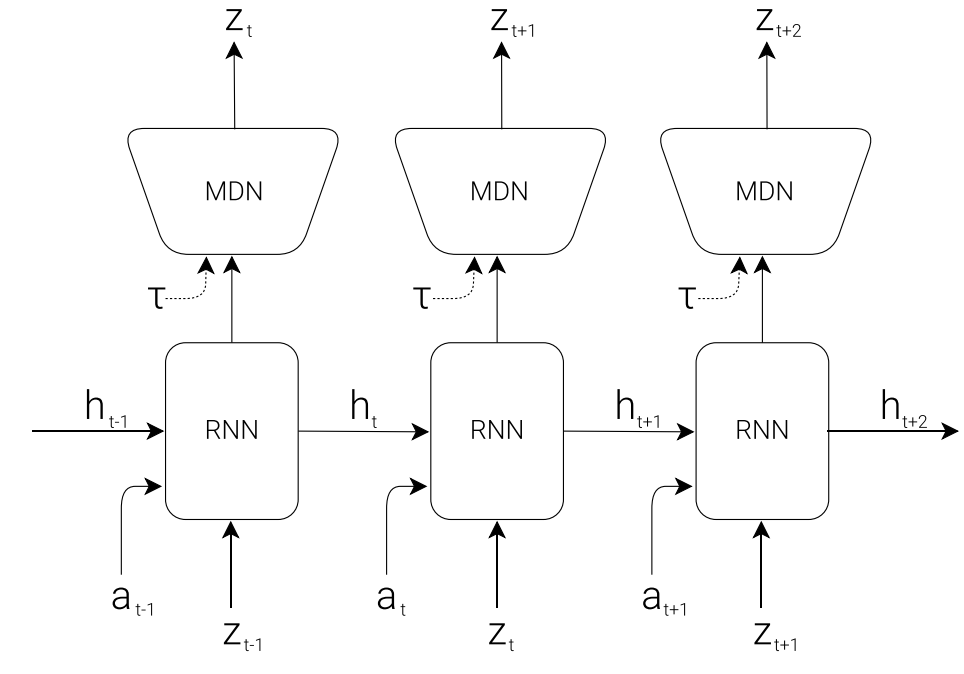
\includegraphics[width=0.75\columnwidth]{sections/4rlopt/images/mdnrnn.png}
  \caption[Temporally unrolled MDN-RNN]{Structure of an unrolled MDN-RNN. The MDN outputs the parameters of a Gaussian mixture distribution used to sample a prediction of the next latent vector $z_{t+1}$, the MDN is controlled by the temperature parameter $\tau$.}
  \label{fig:rl:mdnrnn}
\end{figure}

A constraint of using RNNs is that they expect a fixed sized input sequence. However, in our work, both the shape of the latent state tensor, and the number of actions performed by the agent in a rollout is variable. As such, we employ a common approach to mitigate this problem is by prepending zero values to the input sequence until the desired length is reached, commonly referred to as padding. After performing inference on the model and retrieving the predicted state, we mask the results based on the input padding to ensure we only use valid predictions to select the next action using the controller.

\subsubsection{MDN-RNN}

By combining the mixture density and recurrent networks, we can use rollouts of the environment sampled using a random agent to train the combined network, called an MDN-RNN. We use the network to model $P(z_{t+1}~|~a_t, z_t, h_t)$, where $z_t$, $z_{t+1}$ is the latent state at the times $t$ and $t+1$ respectively, $a_t$ is the action taken at time $t$, and $h_t$ is the hidden state from the RNN network at time $t$. Figure \ref{fig:rl:mdnrnn} shows the combination of the RNN and MDN networks and how we calculate the predictions of the next latent state in sequence.

Furthermore, after training the world model, we must train an agent (or controller) to perform actions in the world model and learn to take optimal actions that maximise reward. During inference of the world model, we use a softmax layer which outputs $\pi$ in the form of a categorial probability distribution which we sample under the Gaussian model parameterised by $(\mu_i, \sigma_i)$.

In figure \ref{fig:rl:mdnrnn} we show that one of the inputs to the MDN is $\tau$, the temperature. By altering the temperature it allows us to control the stochasticity of the agent during training of the controller. The logits of the RNN that represent the predictions for the values of $\pi$ are divided by the temperature prior to being passed into the softmax function which converts the logits into pseudo-probabilities. We incorporate the temperature, $\tau$, into the softmax function using the following equation.

$$
\text{softmax}(\mathbf{x}_i) = \frac{\exp\left( \nicefrac{x_i}{t} \right) }{\Sigma_j \exp \left( \nicefrac{x_j}{t} \right) }
$$

Typically, temperature is a real number in the range $\tau \in \left( 0, \ldots, 1 \right)$, where a value of zero leads to completely deterministic predictions generated by the RNN, whereas larger values introduces a greater amount of stochasticity in the predictions. As larger values of $\tau$ increases the probability of samples with a lower sampling likelihood being selected it leads to a greater diversity of actions taken by the agent in the environment. Importantly, Ha et al. \cite{ha2018worldmodels} found that having a large temperature can aid in preventing the agent from finding strategies to exploit inadequacies in the world model.

\subsection{Action Controller}
